% Standalone TikZ figure: ParseRE pipeline overview.
% Linear left-to-right flow. Data artifacts in rectangles, processing steps in rounded rectangles.
% Replaces the broken figure that had an arrow vanishing into an ellipse.
\documentclass[tikz,border=10pt]{standalone}
\usepackage{tikz}
\usepackage{xcolor}
\usetikzlibrary{positioning,arrows.meta,calc,shapes.geometric}

\definecolor{datacol}{HTML}{F0EFE8}
\definecolor{datacoldark}{HTML}{C8C5B5}
\definecolor{opcol}{HTML}{EAD9C9}
\definecolor{opcoldark}{HTML}{C8997A}
\definecolor{outcol}{HTML}{D4E2C8}
\definecolor{outcoldark}{HTML}{8DAE6A}

\begin{document}
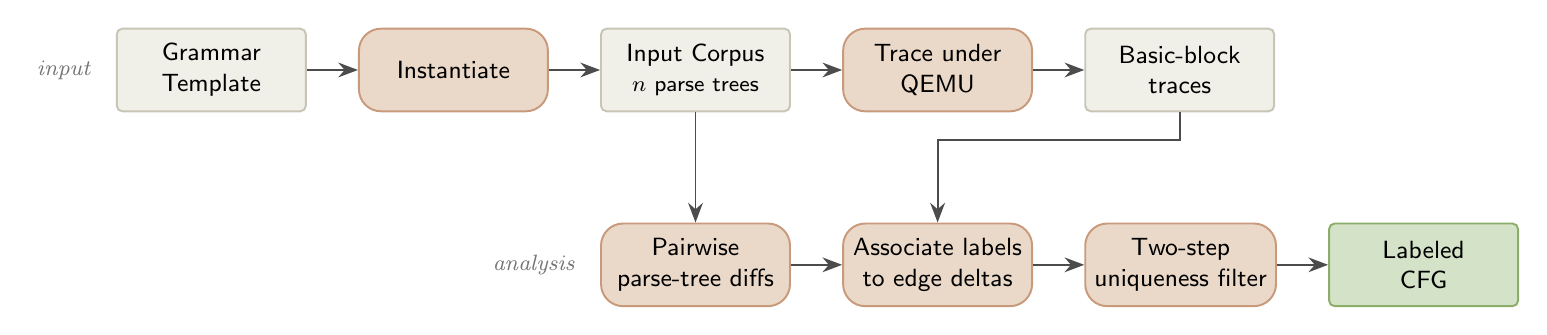
\begin{tikzpicture}[
  font=\sffamily\small,
  node distance=0.65cm,
  data/.style={
    draw=datacoldark, fill=datacol, line width=0.7pt,
    rounded corners=2pt, minimum height=1.05cm, minimum width=2.4cm, align=center,
  },
  op/.style={
    draw=opcoldark, fill=opcol, line width=0.7pt,
    rounded corners=8pt, minimum height=1.05cm, minimum width=2.4cm, align=center,
  },
  outdata/.style={
    draw=outcoldark, fill=outcol, line width=0.7pt,
    rounded corners=2pt, minimum height=1.05cm, minimum width=2.4cm, align=center,
  },
  arrow/.style={-{Stealth[length=2.5mm]}, line width=0.7pt, draw=black!70},
  caption/.style={font=\footnotesize\itshape, text=black!55}
]

% Row 1: input pipeline
\node[data] (template) {Grammar\\Template};
\node[op, right=of template] (inst) {Instantiate};
\node[data, right=of inst] (corpus) {Input Corpus\\\footnotesize $n$ parse trees};
\node[op, right=of corpus] (trace) {Trace under\\QEMU};
\node[data, right=of trace] (traces) {Basic-block\\traces};

% Row 2: analysis pipeline (positioned below corpus)
\node[op, below=1.4cm of corpus] (diff) {Pairwise\\parse-tree diffs};
\node[op, right=of diff] (assoc) {Associate labels\\to edge deltas};
\node[op, right=of assoc] (filter) {Two-step\\uniqueness filter};
\node[outdata, right=of filter] (result) {Labeled\\CFG};

% Horizontal arrows row 1
\draw[arrow] (template) -- (inst);
\draw[arrow] (inst) -- (corpus);
\draw[arrow] (corpus) -- (trace);
\draw[arrow] (trace) -- (traces);

% Vertical bridge: corpus feeds diff
\draw[arrow] (corpus.south) -- ++(0,-0.35) -| (diff.north);

% Vertical bridge: traces feed assoc
\draw[arrow] (traces.south) -- ++(0,-0.35) -| (assoc.north);

% Horizontal arrows row 2
\draw[arrow] (diff) -- (assoc);
\draw[arrow] (assoc) -- (filter);
\draw[arrow] (filter) -- (result);

% Stage labels
\node[caption, left=0.2cm of template] {input};
\node[caption, left=0.2cm of diff] {analysis};

\end{tikzpicture}
\end{document}
